% !TeX program = pdflatex
% !BIB program = bibtex
% Template LaTeX file for DAFx-19 papers

%------------------------------------------------------------------------------------------
%  !  !  !  !  !  !  !  !  !  !  !  ! user defined variables  !  !  !  !  !  !  !  !  !  !  !  !  !  !
% Please use these commands to define title and author(s) of the paper:
\def\papertitle{Waterbottle Synthesis with Modal Signal Processing}
\def\paperauthorA{Elliot K. Canfield-Dafilou, Mark Rau, Jatin Chowdhury}

% Authors' affiliations have to be set below

%------------------------------------------------------------------------------------------
\documentclass[twoside,a4paper]{article}
\usepackage{etoolbox}
\usepackage{dafx_20}
\usepackage{amsmath,amssymb,amsfonts,amsthm}
\usepackage{euscript}
\usepackage[latin1]{inputenc}
\usepackage[T1]{fontenc}
\usepackage{ifpdf}

\usepackage[english]{babel}
\usepackage{caption}
\usepackage{subfig} % or can use subcaption package
\usepackage{xcolor}

\input glyphtounicode
\pdfgentounicode=1

\setcounter{page}{1}
\ninept

% build the list of authors and set the flag \multipleauth to handle the et al. in the copyright note (in DAFx_20.sty)
%==============================DO NOT MODIFY =======================================
\newcounter{numauth}\setcounter{numauth}{1}
\newcounter{listcnt}\setcounter{listcnt}{1}
\newcommand\authcnt[1]{\ifdefined#1 \stepcounter{numauth} \fi}

\newcommand\addauth[1]{
\ifdefined#1 
\stepcounter{listcnt}
\ifnum \value{listcnt}<\value{numauth}
\appto\authorslist{, #1}
\else
\appto\authorslist{~and~#1}
\fi
\fi}
%======DO NOT MODIFY UNLESS YOUR PAPER HAS MORE THAN 10 AUTHORS========================
%==we count the authors defined at the beginning of the file (paperauthorA is mandatory and already accounted for)
\authcnt{\paperauthorB}
\authcnt{\paperauthorC}
\authcnt{\paperauthorD}
\authcnt{\paperauthorE}
\authcnt{\paperauthorF}
\authcnt{\paperauthorG}
\authcnt{\paperauthorH}
\authcnt{\paperauthorI}
\authcnt{\paperauthorJ}
%==we create a list of authors for pdf tagging, for example: paperauthorA, paperauthorB, ... and paperauthorF (last author)
\def\authorslist{\paperauthorA}
\addauth{\paperauthorB}
\addauth{\paperauthorC}
\addauth{\paperauthorD}
\addauth{\paperauthorE}
\addauth{\paperauthorF}
\addauth{\paperauthorG}
\addauth{\paperauthorH}
\addauth{\paperauthorI}
\addauth{\paperauthorJ}
%====================================================================================

\usepackage{times}
% Saves a lot of ouptut space in PDF... after conversion with the distiller
% Delete if you cannot get PS fonts working on your system.

% pdf-tex settings: detect automatically if run by latex or pdflatex
\newif\ifpdf
\ifx\pdfoutput\relax
\else
   \ifcase\pdfoutput
      \pdffalse
   \else
      \pdftrue
\fi

\ifpdf % compiling with pdflatex
  \usepackage[pdftex,
    pdftitle={\papertitle},
    pdfauthor={\paperauthorA},
    colorlinks=false, % links are activated as colror boxes instead of color text
    bookmarksnumbered, % use section numbers with bookmarks
    pdfstartview=XYZ % start with zoom=100% instead of full screen; especially useful if working with a big screen :-)
  ]{hyperref}
  \pdfcompresslevel=9
  \usepackage[pdftex]{graphicx}
%   \usepackage[figure,table]{hypcap}
\else % compiling with latex
  \usepackage[dvips]{epsfig,graphicx}
  \usepackage[dvips,
    colorlinks=false, % no color links
    bookmarksnumbered, % use section numbers with bookmarks
    pdfstartview=XYZ % start with zoom=100% instead of full screen
  ]{hyperref}
  % hyperrefs are active in the pdf file after conversion
  % \usepackage[figure,table]{hypcap}
\fi
\usepackage[hypcap=true]{caption}

% My packages
\usepackage{tikz}
\usepackage{tkz-euclide}
\usetkzobj{all}
\usepackage{cleveref}

\usepackage{listings}
\definecolor{codegreen}{rgb}{0,0.6,0}
\definecolor{codegray}{rgb}{0.5,0.5,0.5}
\definecolor{codepurple}{rgb}{0.58,0,0.82}
\definecolor{backcolour}{rgb}{0.95,0.95,0.92}
 
\lstdefinestyle{mystyle}{
    backgroundcolor=\color{backcolour},   
    commentstyle=\color{codegreen},
    keywordstyle=\color{magenta},
    numberstyle=\tiny\color{codegray},
    stringstyle=\color{codepurple},
    basicstyle=\footnotesize,
    columns=flexible,
    breakatwhitespace=false,         
    breaklines=true,                 
    captionpos=b,                    
    keepspaces=true,                               
    showspaces=false,                
    showstringspaces=false,
    showtabs=false,                  
    tabsize=4
}
 
\lstset{style=mystyle}

\DeclareMathAlphabet{\mathpzc}{OT1}{pzc}{m}{it}
\newcommand{\z}{\mathpzc{z}}

\title{\papertitle}

\affiliation{
\paperauthorA \, }
{\href{http://ccrma.stanford.edu}{Center for Computer Research in Music and Acoustics} \\ Stanford University \\ Palo Alto, CA \\ {\tt\{kermit|mrau|jatin\}@ccrma.stanford.edu}}

\begin{document}
% more pdf-tex settings:
\ifpdf % used graphic file format for pdflatex
  \DeclareGraphicsExtensions{.png,.jpg,.pdf}
\else  % used graphic file format for latex
  \DeclareGraphicsExtensions{.eps}
\fi

\maketitle
%
\begin{abstract}
We present a method for accurately synthesizing the acoustic response
of a waterbottle using modal decomposition.
\end{abstract}

\section{Introduction} \label{sec:intro}
%
Previous works have examined the use of modal signal processing
for synthesizing carillon bells
\cite{canfielddafilou:werner:bellEffects:2017,rau:das:canfielddafilou:carillon:2019},
artificial reverberation \cite{abel2014a}, cymbal synthesis \cite{travis_cymbals},
and more \cite{abel_kurt_modal}.
In this paper, we extend this previous work to use modal Synthesis
for the accurate modelling of waterbottle acoustics. Waterbottles are
particularly well-suited for modal modelling since they have inharmonic
partials. Further, certain waterbottles have been known to have a
pleasing acoustic response, while others sound notably worse.
Additionally, the acoustic response of a waterbottle changes
depending on the amount and the type of liquid contained within, as
well as the potential placement of stickers on the exterior of the bottle.
In this writing, we take measurements from a 32 oz. Wide Mouth
HydroFlask\footnote{\url{https://www.hydroflask.com/32-oz-wide-mouth/color,cobalt,a,92,o,53}},
compared to the waterbottle given to attendees of the 2019 DAFx
conference, measured containing different amounts of water and maple
syrup, as well different placements of stickers on the exteriors of the
bottles.
\newline\newline
The structure of the paper is as follows \dots.

\section{Measurements} \label{sec:measure}
%
Talk about measurements \dots
%
\begin{figure}[!htb]
    \centering
    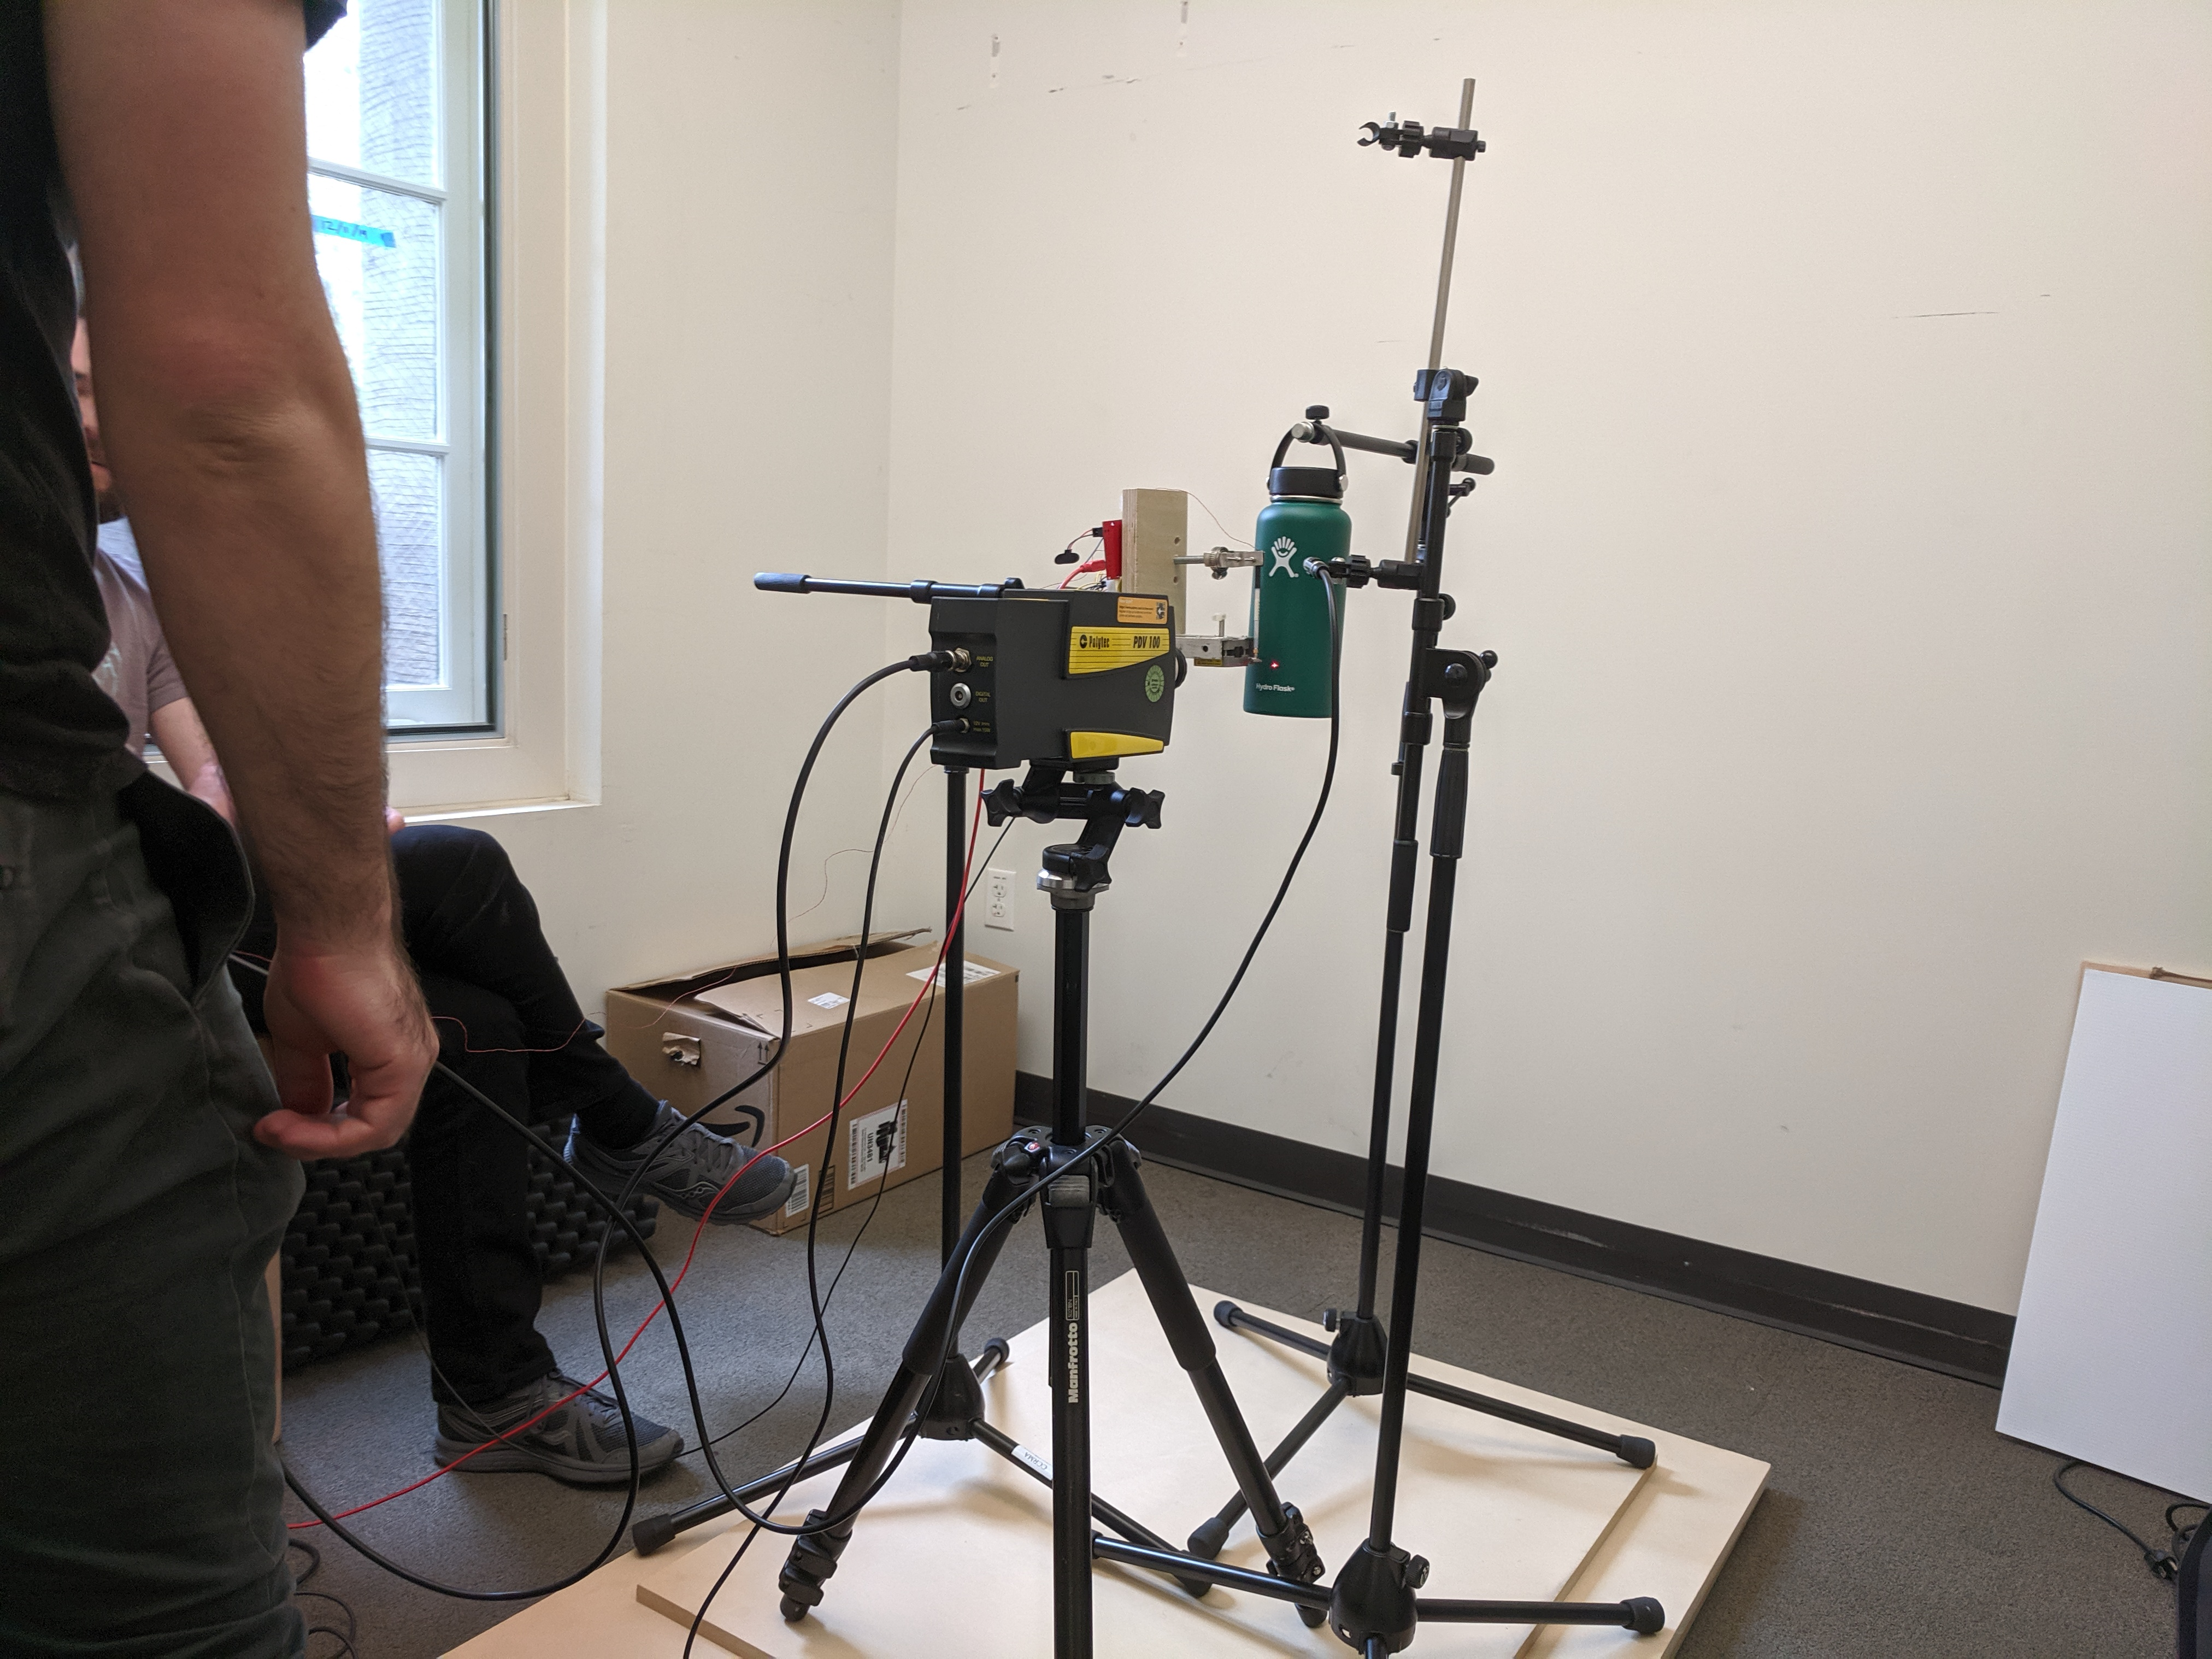
\includegraphics[width=3in]{Figures/hydroflask_measure}
    \caption{\it{Measurement setup for the HydroFlask waterbottle}}
    \label{fig:hydro_measure}
\end{figure}
%
\begin{figure}[!htb]
    \centering
    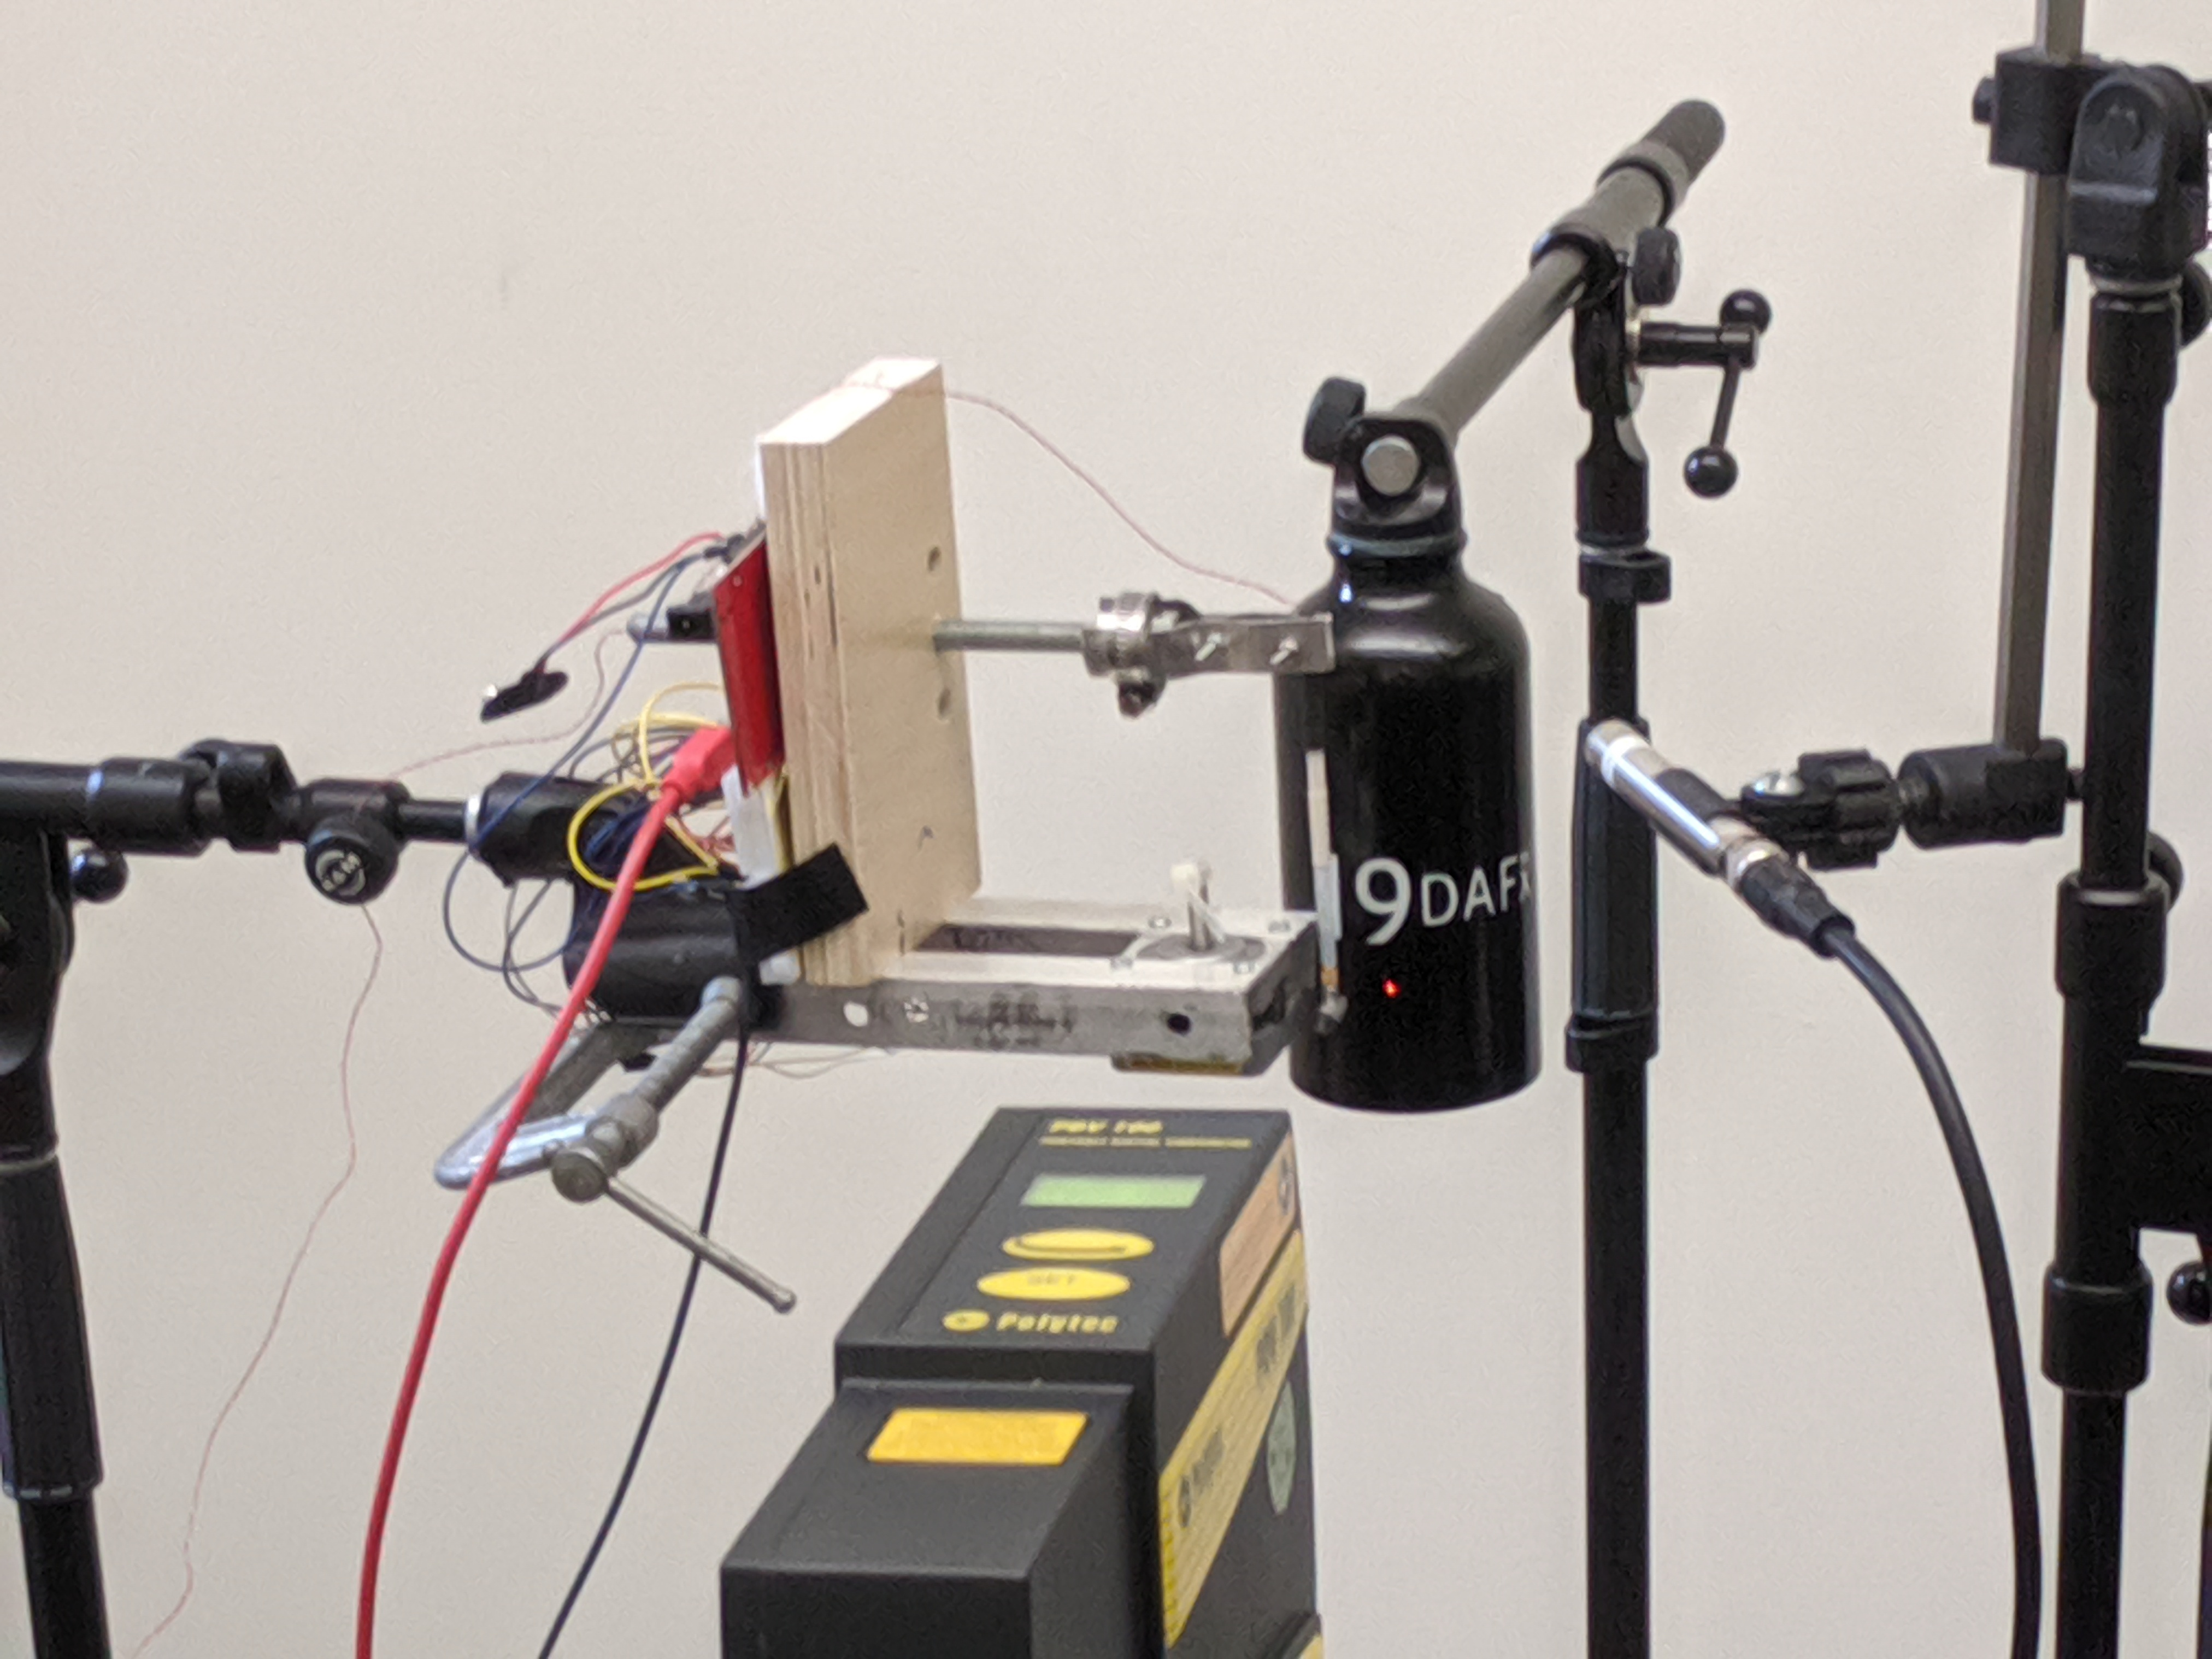
\includegraphics[width=3in]{Figures/dafx_measure}
    \caption{\it{Measurement setup for the DAFx waterbottle}}
    \label{fig:dafx_measure}
\end{figure}

\section{Analysis} \label{sec:analysis}
%
For modal analysis we use the method described in
\cite{canfielddafilou:werner:bellEffects:2017}, using helper functions
provided by the \texttt{Python} audio signal processing library
\texttt{audio\_dspy}\footnote{\url{https://github.com/jatinchowdhury18/audio_dspy}}.
This process involves the following steps:
\begin{enumerate}
    \item Picking the modal frequencies from the original recording.
    \item Estimate the decay rate of each mode.
    \item Estimate the complex amplitude of each mode.
\end{enumerate}
%
The process is shown in  full in \cref{fig:modal_analysis}.
\newline\newline
For finding the mode frequencies, we use a simple peak picking
algorithm over the Fourier Transform of the original signal.
\newline\newline
For estimating the mode decay rates, we begin by filtering
the signal using a 4th order Butterworth bandpass filter
centered on the mode frequency, with a bandwidth of 30 Hz.
We then apply a Root-Mean-Squared level detector as defined
in \cite{giannoulis2012compressor} to estimate the energy
envelope of the mode. Finally, we use a linear regression
to estimate the slope of the energy envelope (measured in
Decibels). The slope can be used to find a decay
factor $\tau$ such that the mode decays by a factor of
$e^{-1/\tau}$ every sample.
\newline\newline
After computing the mode frequencies and decay
rate, we can do a simple least squares fit to
estimate the complex amplitude of each mode that
most accurately resynthesizes the original recording.
\newline\newline
Finally, for synthesizing each mode we use the Max Matthews
phasor filter, as introduced in \cite{phasorfilter}.
This filter is described by the difference equation:
\begin{equation}
    y[n] = A x[n] + e^{j\omega} e^{-1/\tau} y[n-1]
\end{equation}
%
where $\tau$ is the mode decay rate described above, $A$ is
the cocmplex amplitude of the mode, and $\omega$ is the mode
frequency.


\begin{figure*}
    \centering
    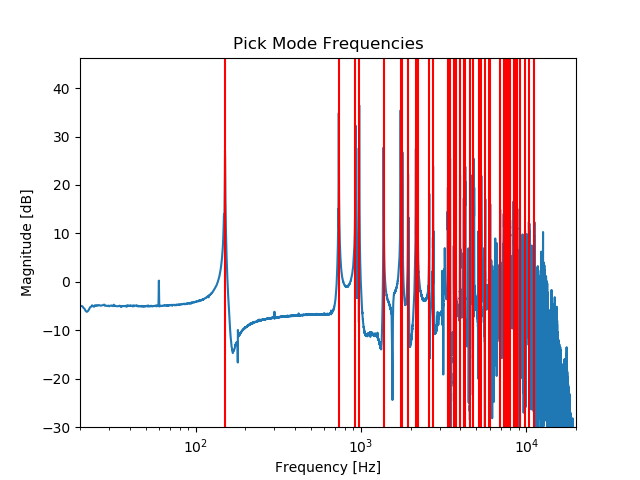
\includegraphics[width=2.25in]{Figures/ModePick_ex}
    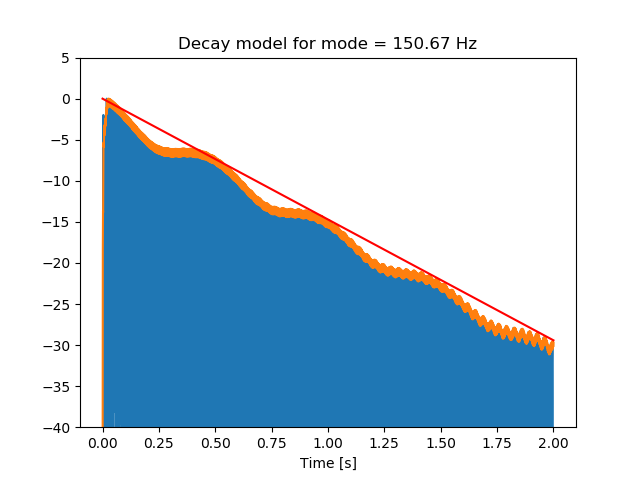
\includegraphics[width=2.25in]{Figures/DecayFit_ex}
    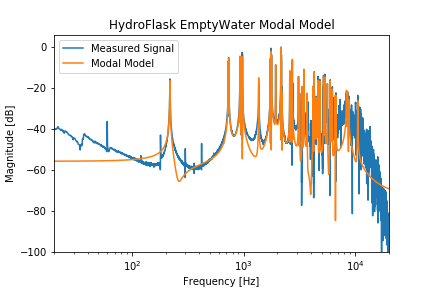
\includegraphics[width=2.25in]{../Figures/HydroFlask/empty}
    \caption{\it{Modal analysis pipeline: (left) picking the mode frequencies,
    (center) estimating the decay rate of a single mode,
    (right) using least-squares to estimate the complex
    amplitudes of the modes that ideally resynthesize the
    original signal.}}
    \label{fig:modal_analysis}
\end{figure*}

%\newpage
\nocite{*}
\bibliographystyle{IEEEbib}
\bibliography{references}

\end{document}
